
%% bare_conf.tex
%% V1.4b
%% 2015/08/26
%% by Michael Shell
%% See:
%% http://www.michaelshell.org/
%% for current contact information.
%%
%% This is a skeleton file demonstrating the use of IEEEtran.cls
%% (requires IEEEtran.cls version 1.8b or later) with an IEEE
%% conference paper.
%%
%% Support sites:
%% http://www.michaelshell.org/tex/ieeetran/
%% http://www.ctan.org/pkg/ieeetran
%% and
%% http://www.ieee.org/

%%*************************************************************************
%% Legal Notice:
%% This code is offered as-is without any warranty either expressed or
%% implied; without even the implied warranty of MERCHANTABILITY or
%% FITNESS FOR A PARTICULAR PURPOSE!
%% User assumes all risk.
%% In no event shall the IEEE or any contributor to this code be liable for
%% any damages or losses, including, but not limited to, incidental,
%% consequential, or any other damages, resulting from the use or misuse
%% of any information contained here.
%%
%% All comments are the opinions of their respective authors and are not
%% necessarily endorsed by the IEEE.
%%
%% This work is distributed under the LaTeX Project Public License (LPPL)
%% ( http://www.latex-project.org/ ) version 1.3, and may be freely used,
%% distributed and modified. A copy of the LPPL, version 1.3, is included
%% in the base LaTeX documentation of all distributions of LaTeX released
%% 2003/12/01 or later.
%% Retain all contribution notices and credits.
%% ** Modified files should be clearly indicated as such, including  **
%% ** renaming them and changing author support contact information. **
%%*************************************************************************


% *** Authors should verify (and, if needed, correct) their LaTeX system  ***
% *** with the testflow diagnostic prior to trusting their LaTeX platform ***
% *** with production work. The IEEE's font choices and paper sizes can   ***
% *** trigger bugs that do not appear when using other class files.       ***                          ***
% The testflow support page is at:
% http://www.michaelshell.org/tex/testflow/



\documentclass[conference]{IEEEtran}
% Some Computer Society conferences also require the compsoc mode option,
% but others use the standard conference format.
%
% If IEEEtran.cls has not been installed into the LaTeX system files,
% manually specify the path to it like:
% \documentclass[conference]{../sty/IEEEtran}

\usepackage{algorithm2e}

 % Перевод плагина
\SetKwInput{KwData}{Input parameters}
\SetKwInput{KwResult}{Result}
\SetKwInput{KwIn}{Input data}
\SetKwInput{KwOut}{Output Data}
\SetKwIF{If}{ElseIf}{Else}{if}{then}{else\ if}{else}{end\ of\ condition}
\SetKwFor{While}{while}{execute}{end\ of\ loop}
\SetKw{KwTo}{to}
\SetKw{KwRet}{return}
\SetKw{Return}{return}
\SetKwBlock{Begin}{begin\ block}{end\ block}
\SetKwSwitch{Switch}{Case}{Other}{Check\ a\ value}{and\ execute}{a\ case}{otherwise}{end\ of\ case}{end\ of\ value\ check}
\SetKwFor{For}{loop}{execute}{end\ of\ loop}
\SetKwFor{ForEach}{for\ each}{execute}{end\ of\ loop}
\SetKwRepeat{Repeat}{repeat}{while}
\SetAlgorithmName{Algorithm}{algorithm}{List of algorithms}


% Some very useful LaTeX packages include:
% (uncomment the ones you want to load)


% *** MISC UTILITY PACKAGES ***
%
%\usepackage{ifpdf}
% Heiko Oberdiek's ifpdf.sty is very useful if you need conditional
% compilation based on whether the output is pdf or dvi.
% usage:
% \ifpdf
%   % pdf code
% \else
%   % dvi code
% \fi
% The latest version of ifpdf.sty can be obtained from:
% http://www.ctan.org/pkg/ifpdf
% Also, note that IEEEtran.cls V1.7 and later provides a builtin
% \ifCLASSINFOpdf conditional that works the same way.
% When switching from latex to pdflatex and vice-versa, the compiler may
% have to be run twice to clear warning/error messages.






% *** CITATION PACKAGES ***
%
%\usepackage{cite}
% cite.sty was written by Donald Arseneau
% V1.6 and later of IEEEtran pre-defines the format of the cite.sty package
% \cite{} output to follow that of the IEEE. Loading the cite package will
% result in citation numbers being automatically sorted and properly
% "compressed/ranged". e.g., [1], [9], [2], [7], [5], [6] without using
% cite.sty will become [1], [2], [5]--[7], [9] using cite.sty. cite.sty's
% \cite will automatically add leading space, if needed. Use cite.sty's
% noadjust option (cite.sty V3.8 and later) if you want to turn this off
% such as if a citation ever needs to be enclosed in parenthesis.
% cite.sty is already installed on most LaTeX systems. Be sure and use
% version 5.0 (2009-03-20) and later if using hyperref.sty.
% The latest version can be obtained at:
% http://www.ctan.org/pkg/cite
% The documentation is contained in the cite.sty file itself.






% *** GRAPHICS RELATED PACKAGES ***
%
\ifCLASSINFOpdf
  \usepackage[pdftex]{graphicx}
  % declare the path(s) where your graphic files are
  % \graphicspath{{../pdf/}{../jpeg/}}
  % and their extensions so you won't have to specify these with
  % every instance of \includegraphics
  % \DeclareGraphicsExtensions{.pdf,.jpeg,.png}
\else
  % or other class option (dvipsone, dvipdf, if not using dvips). graphicx
  % will default to the driver specified in the system graphics.cfg if no
  % driver is specified.
  % \usepackage[dvips]{graphicx}
  % declare the path(s) where your graphic files are
  % \graphicspath{{../eps/}}
  % and their extensions so you won't have to specify these with
  % every instance of \includegraphics
  % \DeclareGraphicsExtensions{.eps}
\fi
% graphicx was written by David Carlisle and Sebastian Rahtz. It is
% required if you want graphics, photos, etc. graphicx.sty is already
% installed on most LaTeX systems. The latest version and documentation
% can be obtained at:
% http://www.ctan.org/pkg/graphicx
% Another good source of documentation is "Using Imported Graphics in
% LaTeX2e" by Keith Reckdahl which can be found at:
% http://www.ctan.org/pkg/epslatex
%
% latex, and pdflatex in dvi mode, support graphics in encapsulated
% postscript (.eps) format. pdflatex in pdf mode supports graphics
% in .pdf, .jpeg, .png and .mps (metapost) formats. Users should ensure
% that all non-photo figures use a vector format (.eps, .pdf, .mps) and
% not a bitmapped formats (.jpeg, .png). The IEEE frowns on bitmapped formats
% which can result in "jaggedy"/blurry rendering of lines and letters as
% well as large increases in file sizes.
%
% You can find documentation about the pdfTeX application at:
% http://www.tug.org/applications/pdftex





% *** MATH PACKAGES ***
%
%\usepackage{amsmath}
% A popular package from the American Mathematical Society that provides
% many useful and powerful commands for dealing with mathematics.
%
% Note that the amsmath package sets \interdisplaylinepenalty to 10000
% thus preventing page breaks from occurring within multiline equations. Use:
%\interdisplaylinepenalty=2500
% after loading amsmath to restore such page breaks as IEEEtran.cls normally
% does. amsmath.sty is already installed on most LaTeX systems. The latest
% version and documentation can be obtained at:
% http://www.ctan.org/pkg/amsmath





% *** SPECIALIZED LIST PACKAGES ***
%
%\usepackage{algorithmic}
% algorithmic.sty was written by Peter Williams and Rogerio Brito.
% This package provides an algorithmic environment fo describing algorithms.
% You can use the algorithmic environment in-text or within a figure
% environment to provide for a floating algorithm. Do NOT use the algorithm
% floating environment provided by algorithm.sty (by the same authors) or
% algorithm2e.sty (by Christophe Fiorio) as the IEEE does not use dedicated
% algorithm float types and packages that provide these will not provide
% correct IEEE style captions. The latest version and documentation of
% algorithmic.sty can be obtained at:
% http://www.ctan.org/pkg/algorithms
% Also of interest may be the (relatively newer and more customizable)
% algorithmicx.sty package by Szasz Janos:
% http://www.ctan.org/pkg/algorithmicx




% *** ALIGNMENT PACKAGES ***
%
%\usepackage{array}
% Frank Mittelbach's and David Carlisle's array.sty patches and improves
% the standard LaTeX2e array and tabular environments to provide better
% appearance and additional user controls. As the default LaTeX2e table
% generation code is lacking to the point of almost being broken with
% respect to the quality of the end results, all users are strongly
% advised to use an enhanced (at the very least that provided by array.sty)
% set of table tools. array.sty is already installed on most systems. The
% latest version and documentation can be obtained at:
% http://www.ctan.org/pkg/array


% IEEEtran contains the IEEEeqnarray family of commands that can be used to
% generate multiline equations as well as matrices, tables, etc., of high
% quality.




% *** SUBFIGURE PACKAGES ***
%\ifCLASSOPTIONcompsoc
%  \usepackage[caption=false,font=normalsize,labelfont=sf,textfont=sf]{subfig}
%\else
%  \usepackage[caption=false,font=footnotesize]{subfig}
%\fi
% subfig.sty, written by Steven Douglas Cochran, is the modern replacement
% for subfigure.sty, the latter of which is no longer maintained and is
% incompatible with some LaTeX packages including fixltx2e. However,
% subfig.sty requires and automatically loads Axel Sommerfeldt's caption.sty
% which will override IEEEtran.cls' handling of captions and this will result
% in non-IEEE style figure/table captions. To prevent this problem, be sure
% and invoke subfig.sty's "caption=false" package option (available since
% subfig.sty version 1.3, 2005/06/28) as this is will preserve IEEEtran.cls
% handling of captions.
% Note that the Computer Society format requires a larger sans serif font
% than the serif footnote size font used in traditional IEEE formatting
% and thus the need to invoke different subfig.sty package options depending
% on whether compsoc mode has been enabled.
%
% The latest version and documentation of subfig.sty can be obtained at:
% http://www.ctan.org/pkg/subfig




% *** FLOAT PACKAGES ***
%
%\usepackage{fixltx2e}
% fixltx2e, the successor to the earlier fix2col.sty, was written by
% Frank Mittelbach and David Carlisle. This package corrects a few problems
% in the LaTeX2e kernel, the most notable of which is that in current
% LaTeX2e releases, the ordering of single and double column floats is not
% guaranteed to be preserved. Thus, an unpatched LaTeX2e can allow a
% single column figure to be placed prior to an earlier double column
% figure.
% Be aware that LaTeX2e kernels dated 2015 and later have fixltx2e.sty's
% corrections already built into the system in which case a warning will
% be issued if an attempt is made to load fixltx2e.sty as it is no longer
% needed.
% The latest version and documentation can be found at:
% http://www.ctan.org/pkg/fixltx2e


%\usepackage{stfloats}
% stfloats.sty was written by Sigitas Tolusis. This package gives LaTeX2e
% the ability to do double column floats at the bottom of the page as well
% as the top. (e.g., "\begin{figure*}[!b]" is not normally possible in
% LaTeX2e). It also provides a command:
%\fnbelowfloat
% to enable the placement of footnotes below bottom floats (the standard
% LaTeX2e kernel puts them above bottom floats). This is an invasive package
% which rewrites many portions of the LaTeX2e float routines. It may not work
% with other packages that modify the LaTeX2e float routines. The latest
% version and documentation can be obtained at:
% http://www.ctan.org/pkg/stfloats
% Do not use the stfloats baselinefloat ability as the IEEE does not allow
% \baselineskip to stretch. Authors submitting work to the IEEE should note
% that the IEEE rarely uses double column equations and that authors should try
% to avoid such use. Do not be tempted to use the cuted.sty or midfloat.sty
% packages (also by Sigitas Tolusis) as the IEEE does not format its papers in
% such ways.
% Do not attempt to use stfloats with fixltx2e as they are incompatible.
% Instead, use Morten Hogholm'a dblfloatfix which combines the features
% of both fixltx2e and stfloats:
%
% \usepackage{dblfloatfix}
% The latest version can be found at:
% http://www.ctan.org/pkg/dblfloatfix




% *** PDF, URL AND HYPERLINK PACKAGES ***
%
%\usepackage{url}
% url.sty was written by Donald Arseneau. It provides better support for
% handling and breaking URLs. url.sty is already installed on most LaTeX
% systems. The latest version and documentation can be obtained at:
% http://www.ctan.org/pkg/url
% Basically, \url{my_url_here}.




% *** Do not adjust lengths that control margins, column widths, etc. ***
% *** Do not use packages that alter fonts (such as pslatex).         ***
% There should be no need to do such things with IEEEtran.cls V1.6 and later.
% (Unless specifically asked to do so by the journal or conference you plan
% to submit to, of course. )


% correct bad hyphenation here
\hyphenation{op-tical net-works semi-conduc-tor}

% FIXME Remove, when got ready to publish
\usepackage[usenames,dvipsnames,svgnames,table]{xcolor}
\definecolor{rclr}{rgb}{0.5,0.1,0.1}
\definecolor{eclr}{rgb}{0,0.5,0.5}
\colorlet{acolor}{blue}
\colorlet{rcolor}{red}
\definecolor{ncolor}{rgb}{0.5,0.5,0.1}
\newcommand{\aaa}[2][acolor]{\noindent\textcolor{eclr}%
{+\ [}\textcolor{#1}{#2}\textcolor{eclr}{]}}
\newcommand{\rrr}[2][rcolor]{\noindent%
\textcolor{eclr}{-\ [}\textcolor{#1}{#2}\textcolor{eclr}{]}}
\newcommand{\nnn}[2][ncolor]{\noindent%
\textcolor{eclr}{!\ [}\textcolor{#1}{#2}\textcolor{eclr}{]}}

\begin{document}
%
% paper title
% Titles are generally capitalized except for words such as a, an, and, as,
% at, but, by, for, in, nor, of, on, or, the, to and up, which are usually
% not capitalized unless they are the first or last word of the title.
% Linebreaks \\ can be used within to get better formatting as desired.
% Do not put math or special symbols in the title.
\title{Control Flow Graph Visualization for Reverse Engineering of Compiled Software}


% author names and affiliations
% use a multiple column layout for up to three different
% affiliations
\author{\IEEEauthorblockN{Andrey Mikhailov, Aleksey Hmelnov, Evgeny Cherkashin and Igor Bychkov}
\IEEEauthorblockA{Institute of System Dynamics and Control Theory, \\
National Research Irkutsk State Technical University,\\
Irkutsk, Russian Federation\\
\texttt{\{mikhailov,alex,eugeneai,bychkov\}@icc.ru}}
}
% conference papers do not typically use \thanks and this command
% is locked out in conference mode. If really needed, such as for
% the acknowledgment of grants, issue a \IEEEoverridecommandlockouts
% after \documentclass

% for over three affiliations, or if they all won't fit within the width
% of the page, use this alternative format:
%
%\author{\IEEEauthorblockN{Michael Shell\IEEEauthorrefmark{1},
%Homer Simpson\IEEEauthorrefmark{2},
%James Kirk\IEEEauthorrefmark{3},
%Montgomery Scott\IEEEauthorrefmark{3} and
%Eldon Tyrell\IEEEauthorrefmark{4}}
%\IEEEauthorblockA{\IEEEauthorrefmark{1}School of Electrical and Computer Engineering\\
%Georgia Institute of Technology,
%Atlanta, Georgia 30332--0250\\ Email: see http://www.michaelshell.org/contact.html}
%\IEEEauthorblockA{\IEEEauthorrefmark{2}Twentieth Century Fox, Springfield, USA\\
%Email: homer@thesimpsons.com}
%\IEEEauthorblockA{\IEEEauthorrefmark{3}Starfleet Academy, San Francisco, California 96678-2391\\
%Telephone: (800) 555--1212, Fax: (888) 555--1212}
%\IEEEauthorblockA{\IEEEauthorrefmark{4}Tyrell Inc., 123 Replicant Street, Los Angeles, California 90210--4321}}




% use for special paper notices
%\IEEEspecialpapernotice{(Invited Paper)}




% make the title area
\maketitle

% As a general rule, do not put math, special symbols or citations
% in the abstract
\begin{abstract}
Reverse engineering of the compiled software is an important task in software engineering.  One of the stages of reverse engineering technologies is a construction and analysis of control flow graph that reflect a general structure of corresponding algorithms.  The paper presents a technique for analyzing and visualizing the control flow graph of a compiled software.  The analysis is based on semantically equivalent transformations of the original graph resulting in an abstract node that contains a hierarchy of isolated regions, which then associated with predefined templates to form resulting graphical representation.  The templates and additional signature data allow one to recognize the high-level programming structures and statements used, to construct a flow-chart notation of the original program, increasing both the productivity and detail level of the software description.
\end{abstract}

% no keywords




% For peer review papers, you can put extra information on the cover
% page as needed:
% \ifCLASSOPTIONpeerreview
% \begin{center} \bfseries EDICS Category: 3-BBND \end{center}
% \fi
%
% For peerreview papers, this IEEEtran command inserts a page break and
% creates the second title. It will be ignored for other modes.
\IEEEpeerreviewmaketitle

\section{Introduction}

Reverse engineering of the compiled software (a program after processing its source code by a compiler) is an important task in software engineering as it allows one to solve a wide variety of software quality assessment problems, such as productivity of compiled code, quality of compiler and system libraries, peculiarities of hardware architectures the program running on.  Reverse engineering is also used for regain the access to legacy code, whose source counterpart is already lost, and for investigation of virus and malicious program behavior.  One of the main part of any reverse engineering technologies is a construction and analysis of so-called control flow graph that reflect a general structure of corresponding algorithms.  Artificial intelligence techniques such as pattern recognition and rewrite rule engines have extensive use in the analysis.

The control flow graph is a natural representation that can be automatically figured out from the source code of its compiled binaries.  The graph is used by compiler as an intermediate structure for optimizing transformations.  The source code text contains all the necessary information on program behavior.  Its analysis usually is a complex task even with technological support of nowadays integrated development environments, which make it significantly easier.

Binary code analysis is a more complex task, and it requires a wide variety of IT knowledge.  Special software such as disassemblers and decompilers are used for this purpose.  The decompiling of a runtime is in principle an impracticable task: the reconstructed high-level code is more difficult in understanding as compared to its assembler counterpart.  The visual analysis of the control flow is an alternate way.  There are number of visual representation and processing software, which are universal enough, such as uDraw (daVinci)~\cite{10}, VCG~\cite{14}, Graphlet~\cite{12}, GraVis~\cite{13}, Graph Drawing Server~\cite{9}, graphViz~\cite{11}, VisualGraph~\cite{15}.  These systems have a broad toolkits, but visualization and analysis of control flow graph requires a special processing routines.

Algorithms of graph visualization are developed since \nnn{60-ties}~\cite{7}.  The works of P.~Eades~\cite{5}, T.~Kamada~\cite{q1}, and S.~Kawai~\cite{6} considered to be classical in this research field and devoted to universal approaches to graph visualization problems.  The control flow graph is directed and usually visualized by means of layers~\cite{4}.  The process consists of four stages:
\begin{description}
\item [Distribution of graph nodes in a layer.] Each node is assigned a rank.  All directed arcs can connect nodes from a lower rank to a higher one.  Nodes of the same rank cannot be connected with arcs.  Rank distribution of the nodes is performed with various techniques, the simplest one is based on path length calculation in depth-first graph traversal procedure.
\item[Defining order on the nodes of a layer.] The nodes of a layer are ordered according to principle of minimization of intersections of \nnn{the arcs !WE SAID that THERE ARE NO CONNECTIONS of THE NODES OF THE SAME RANK!}.  \nnn{Method of median}~\cite{8} is most widely used technique for solving the problem.
\item[Figuring out of the node coordinates in a layer.] Each node of the each layer is assigned a coordinate so as the graph will correspond to predefined aesthetic criteria.

\item[Arc drawing.] On this stage the arcs are drawn according to \nnn{criteria}, for example, arcs can be indirect lines.
\end{description}

The paper presents a technique for analyzing and visualizing the control flow graph of a compiled software. The analysis is based on semantically equivalent transformations of the original graph resulting in an abstract node that contains a hierarchy of isolated regions, which then associated with predefined templates to form resulting graphical representation.  The templates and additional signature data for library modules allow one to recognize among the subgraphs the high--level programming language structures and statements used, e.g., to construct flow--chart notation of the original program.

\section{Some WONDERFUL basis and theory}

\nnn{According to the technique, program's graph of control flow is separated  on regions having one input and one output node, then the regions are replaced with abstract nodes.}

\subsection{Quality criteria of the control flow graph visualization}

The main criterion of quality of control graph visualization is the correspondence of the image to the nature of the visualized informational object. The quality assessment depends on various structural and systematical characteristics of the object.  Three basis features are emphasized specially among the criteria: \nnn{visual arrangement, aesthetics, restrictions}.
\begin{itemize}
\item \emph{Visual arrangement} \nnn{WE NEED CONSTRUCTIVE DEFINITION!! NOT A CONSTRAINTS!!}
\item \emph{aesthetics}
\item \emph{restrictions}
\end{itemize}

A control flow graph that was reconstructed from a binaries consists of operator block nodes, starting node, and an non-empty set of finish nodes, as well as edges corresponding to transfer of control.  A natural image of the control flow graph is a flowchart diagram.  For the flow charts we define the following \nnn{visual arrangement} for its nodes (Fig.~\ref{fig:blocks}).

\section{Control flow graph visualizing}
\label{sec:cfg-vis}

Nowadays programming languages in most cases contain a standard set of high--level control flow operators (if--then, if--then--else, for, while, etc.).  These operators when compiled produce their specific subgraphs.  For example, if--then operator produces a graph depicted in Fig.~\ref{fig:IfSt}, where ``then'' part could correspond to another control subgraph.
\begin{figure}[htbp]
	\centering
		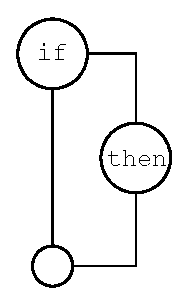
\includegraphics[width=0.15\textwidth]{Pic/Pic2.eps}
	\caption{Subgraph of if--then operator}
	\label{fig:IfSt}
\end{figure}

One can describe a corresponding subgraph for all standard high--level language flow control operators.  Each generated subgraph is described as a template.  The control operators are revealed and reconstructed in whole flow control graph by means of recognition of the templates in the graph and folding the recognized structure into an abstract node.  The arcs going into and from the abstract node are reconnected accordingly.  The reconstruction process is repeated until either the graph folds into one abstract node, and in this case graph is referred to as \emph{\nnn{reducible}}, or there is a subgraph that does not correspond to any of the templates.  In the last case the graph is called \emph{\nnn{inreducible}}, and the subgraph --- \emph{\nnn{indeterminate}}.

Structural high--level programming languages compiler produces only reducible flow control graphs.  This will hold for most of other languages as long as ``goto'' operator is not used explicitly or implicitly.  There are to approaches for overcoming this problem:
\begin{enumerate}
\item Perform an indeterminate subgraph riddance operation.  The essential disadvantage of the approach is the necessity of addition and deletion of nodes and arcs in the graph, this is not allowed in control flow graph model visualization.
\item Recognize the indeterminate subgraph and replace it with an abstract node.  \nnn{Some COMMENT NEEDED whether IT IS GOOD OR BAD.}
\end{enumerate}

\subsection{Algorithm of control flow graph structuring}
\label{sec:algor-contr-flow}

The developed algorithm is based on structural analysis technique proposed in~\cite{17} that suggest to recognize subgraph of a predefined form (a template) and replace them with an abstract node, reassigning arc \nnn{terminals} accordingly.  Template application is carried out in depth-first order until the graph folds into one abstract node.  A tree of dominating nodes is constructed.  The tree is used for arc classification and cycle recognition.  The result quality strongly depends on template application order. The algorithm is as follows:

\begin{algorithm}[h]
\SetAlgoLined %% Connects logical parts with lines
\KwData{G, D, P}
\KwResult{An abstract node containing a hierarchy of folded subgraphs}
%\While{$|E| \neq 0$ и $|V| \neq 1$}{
	\ForEach{$v \in D$ in backward order}{
		\ForEach{$p \in Children(v)$}{
			\If{$p\quad pidom\quad v$}{
				$S \leftarrow Children(v) \setminus p $ \\
				\If{$Classify\_Region(S) \neq \textit{indeterminat}$}{
					$Apply\_Template(S)$
				}\Else{
					$Hierarchical\_Placer(S \cup p)$ \\
					$Recognize\_Indeterminant\_Region(S)$
				}
				$Modify(G,D,P)$
			}
		}
	}
%}
\caption{Algorithm of control flow graph structuring}
\label{alg:struct}
\end{algorithm}

% Line 287 ... FIXME translate paragraph

Traversing of \nnn{the} denominator tree is conducted from leaves to the root in a reverse order with respect to breadth--first strategy.  For this purpose, a stack structure is used.  ....

%line 280 Cannot understand the essence.

As soon as a set of nodes of \nnn{TT--region} (subgraph) is recognized, the region is classified.  The templates (Fig.~\ref{fig:Regions}) are sequentially applied to the recognized \nnn{TT-region}.  If the region corresponds to a template it is considered to be \emph{determined} otherwise \emph{undetermined}.

For the determined subgraphs a new abstract node is constructed.  The node embodies the subgraphs and bounding rectangle of the subgraph calculated according to rules defined in the template.  The Hierarchical \nnn{raskladchik} is applied to the undetermined regions followed by figuring out the bounding rectangle on the base of node coordinates.  The undetermined region is replaced with new abstract node.

Finally, we obtain one abstract region, having no input and output arcs.  The region will contain all the hierarchy of folded subroutines.  The bounding rectangle is figured out for the region.  All graph nodes will be located inside the rectangle.

\begin{figure}[htbp]
	\centering
		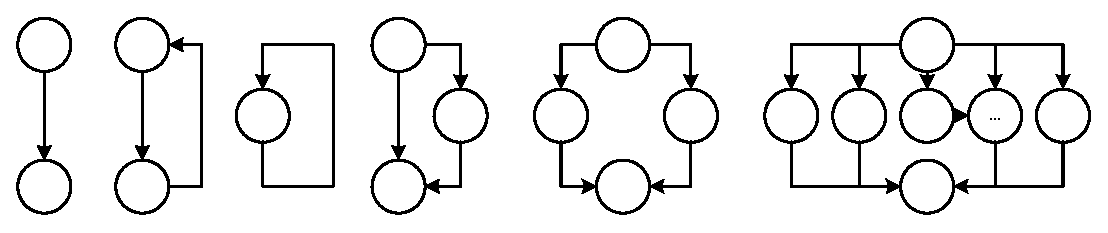
\includegraphics[width=1\textwidth]{Pic/Reg.eps}
	\caption{Applicable templates}
	\label{fig:Regions}
\end{figure}

\subsection{Raskladka process}
\label{sec:raskladka-process}

The R process is carried out recursively from top region down to lower regions.  For the top region initial coordinates is defined.  If a region has a template with visualization rules, the rules are applied.  The example of \texttt{if--then--else} operator is given in Fig.~\ref{fig:IfThenElse}.

\begin{figure}[htbp]
	\centering
		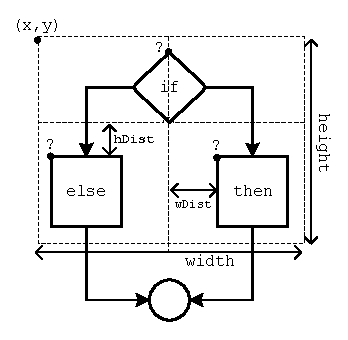
\includegraphics[width=0.4\textwidth]{Pic/IfThenElse.eps}
	\caption{Visualizing template got \texttt{if-then-else} operator}
	\label{fig:IfThenElse}
\end{figure}

The coordinate computation rules for \texttt{if--then--else} operator is as follows:
\begin{itemize}
\item \texttt{if.x = x + abs(width - if.width) / 2};
\item \texttt{then.x = x  + wDist / 2, then.y = y + if.height + hDist};
\item \texttt{else.x = x - else.width - wDist / 2, else.y = y + if.height + hDist};
\end{itemize}
where \texttt{wDist} is a vertical distance between nodes, \texttt{hDist} is a horizontal distance.  These parameters is defined manually and reflect aesthetic criteria.  The visualizing rules are defined analogously for each template.  Thus, the R process is a sequential application of the visualizing rules for the folded regions (subgraphs).

\section{Implementation}
\label{sec:implementation}



\subsubsection{Subsubsection Heading Here}
Subsubsection text here.




% An example of a floating figure using the graphicx package.
% Note that \label must occur AFTER (or within) \caption.
% For figures, \caption should occur after the \includegraphics.
% Note that IEEEtran v1.7 and later has special internal code that
% is designed to preserve the operation of \label within \caption
% even when the captionsoff option is in effect. However, because
% of issues like this, it may be the safest practice to put all your
% \label just after \caption rather than within \caption{}.
%
% Reminder: the "draftcls" or "draftclsnofoot", not "draft", class
% option should be used if it is desired that the figures are to be
% displayed while in draft mode.
%
%\begin{figure}[!t]
%\centering
%\includegraphics[width=2.5in]{myfigure}
% where an .eps filename suffix will be assumed under latex,
% and a .pdf suffix will be assumed for pdflatex; or what has been declared
% via \DeclareGraphicsExtensions.
%\caption{Simulation results for the network.}
%\label{fig_sim}
%\end{figure}

% Note that the IEEE typically puts floats only at the top, even when this
% results in a large percentage of a column being occupied by floats.


% An example of a double column floating figure using two subfigures.
% (The subfig.sty package must be loaded for this to work.)
% The subfigure \label commands are set within each subfloat command,
% and the \label for the overall figure must come after \caption.
% \hfil is used as a separator to get equal spacing.
% Watch out that the combined width of all the subfigures on a
% line do not exceed the text width or a line break will occur.
%
%\begin{figure*}[!t]
%\centering
%\subfloat[Case I]{\includegraphics[width=2.5in]{box}%
%\label{fig_first_case}}
%\hfil
%\subfloat[Case II]{\includegraphics[width=2.5in]{box}%
%\label{fig_second_case}}
%\caption{Simulation results for the network.}
%\label{fig_sim}
%\end{figure*}
%
% Note that often IEEE papers with subfigures do not employ subfigure
% captions (using the optional argument to \subfloat[]), but instead will
% reference/describe all of them (a), (b), etc., within the main caption.
% Be aware that for subfig.sty to generate the (a), (b), etc., subfigure
% labels, the optional argument to \subfloat must be present. If a
% subcaption is not desired, just leave its contents blank,
% e.g., \subfloat[].


% An example of a floating table. Note that, for IEEE style tables, the
% \caption command should come BEFORE the table and, given that table
% captions serve much like titles, are usually capitalized except for words
% such as a, an, and, as, at, but, by, for, in, nor, of, on, or, the, to
% and up, which are usually not capitalized unless they are the first or
% last word of the caption. Table text will default to \footnotesize as
% the IEEE normally uses this smaller font for tables.
% The \label must come after \caption as always.
%
%\begin{table}[!t]
%% increase table row spacing, adjust to taste
%\renewcommand{\arraystretch}{1.3}
% if using array.sty, it might be a good idea to tweak the value of
% \extrarowheight as needed to properly center the text within the cells
%\caption{An Example of a Table}
%\label{table_example}
%\centering
%% Some packages, such as MDW tools, offer better commands for making tables
%% than the plain LaTeX2e tabular which is used here.
%\begin{tabular}{|c||c|}
%\hline
%One & Two\\
%\hline
%Three & Four\\
%\hline
%\end{tabular}
%\end{table}


% Note that the IEEE does not put floats in the very first column
% - or typically anywhere on the first page for that matter. Also,
% in-text middle ("here") positioning is typically not used, but it
% is allowed and encouraged for Computer Society conferences (but
% not Computer Society journals). Most IEEE journals/conferences use
% top floats exclusively.
% Note that, LaTeX2e, unlike IEEE journals/conferences, places
% footnotes above bottom floats. This can be corrected via the
% \fnbelowfloat command of the stfloats package.




\section{Conclusion}
We have proposed and implemented a software tools realizing a new approach to surface graph \nnn{raskladka} on the base of techniques of structural analysis.  The tools have been used for structural ... of attributed graphs.  A probation was performed on CPU2000 test set\footnote{https://www.spec.org/cpu2000/ --- Standard Performance Evaluation Corporation.  SPEC CPU2000 is a test set for assessment of the performance of a central processing unit. The test are used for compiler quality evaluation.} and the following \nnn{generalized} results are obtained:
\begin{itemize}
\item 197.parser (Syntactic parser of a natural language);
\item 252.eon (Ray tracing).
\end{itemize}




The automation of the flow control analysis allows engineer to devote more efforts for description of the templates increasing both the productivity and detail level of the software description.


% conference papers do not normally have an appendix


% use section* for acknowledgment
\section*{Acknowledgment}

\nnn{The results presented in the paper are obtained with partial support of...
The authors would like to thank...}








% trigger a \newpage just before the given reference
% number - used to balance the columns on the last page
% adjust value as needed - may need to be readjusted if
% the document is modified later
%\IEEEtriggeratref{8}
% The "triggered" command can be changed if desired:
%\IEEEtriggercmd{\enlargethispage{-5in}}

% references section

% can use a bibliography generated by BibTeX as a .bbl file
% BibTeX documentation can be easily obtained at:
% http://mirror.ctan.org/biblio/bibtex/contrib/doc/
% The IEEEtran BibTeX style support page is at:
% http://www.michaelshell.org/tex/ieeetran/bibtex/
%\bibliographystyle{IEEEtran}
% argument is your BibTeX string definitions and bibliography database(s)
%\bibliography{IEEEabrv,../bib/paper}
%
% <OR> manually copy in the resultant .bbl file
% set second argument of \begin to the number of references
% (used to reserve space for the reference number labels box)
\begin{thebibliography}{1}

\bibitem{IEEEhowto:kopka}
H.~Kopka and P.~W. Daly, \emph{A Guide to \LaTeX}, 3rd~ed.\hskip 1em plus
  0.5em minus 0.4em\relax Harlow, England: Addison-Wesley, 1999.

\end{thebibliography}




% that's all folks
\end{document}

%%% Local Variables:
%%% mode: latex
%%% TeX-master: t
%%% End:
